\section{Experiments and Results}
\begin{figure*}[t]
 \centering
 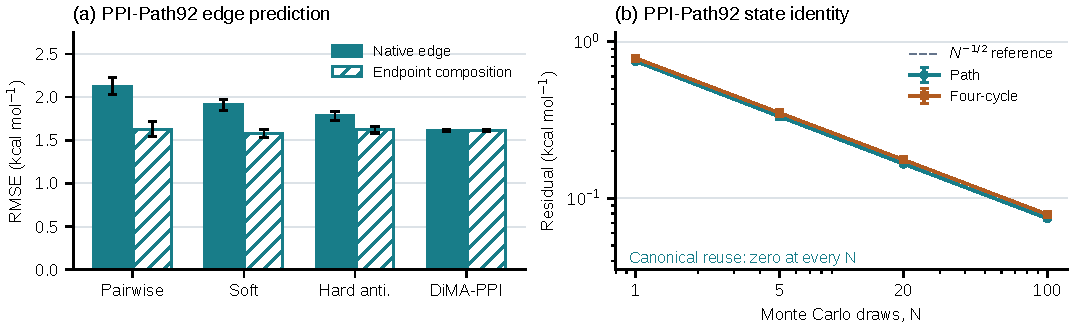
\includegraphics[width=\textwidth]{fig_results.pdf}
 \caption{Evaluation on PPI-Path92. (a) RMSE of native mutant-to-mutant
 predictions and composition of predicted WT effects, evaluated against
 differences of measured WT effects. Bars and error bars denote the mean
 and sample SD across five seeds. (b) Consistency residuals under independent
 state sampling with fixed StaB-ddG parameters. Canonical reuse yields zero
 measured residuals at all sample counts, as indicated below the curves.}
 \label{fig:results}
\end{figure*}
\subsection{Datasets and Evaluation Protocol}
\textbf{S1129.} The public benchmark contains 1,129 single substitutions
from 111 complexes following the two official exclusions from S1131. We use the five predefined complex-disjoint
outer folds from the DSSA-PPI protocol~\cite{dssappi}, with test sizes 169,
142, 271, 252 and 295. Approximately one eighth of each outer training fold
is reserved for validation using a seeded mutation-level split; complexes
may therefore occur in both fitting and validation subsets. We report the mean and sample SD across seeds 42--46 after averaging
per-fold metrics within each seed. PCC, Spearman correlation and RMSE
measure linear association, rank agreement and error magnitude, respectively.

\textbf{PPI-Path92.} We construct the Protein--Protein Interaction Mutation
Path Benchmark (PPI-Path92) from repeated-site measurements in S1129.
Measurements are grouped by complex, chain, PDB site and WT residue. Sites
with at least two distinct measured mutant variants are retained, with
duplicate records resolved by selecting the earliest source row. The resulting benchmark
contains 92 site panels from 27 complexes and 793 amino-acid states.
For each ordered mutant pair, the target is
\begin{equation}
 y^{\rm derived}_{b\to c}=y_{\mathrm{WT}\to c}-y_{\mathrm{WT}\to b}.
 \label{eq:path92target}
\end{equation}
PPI-Path92 contains 9,904 mutant-to-mutant comparisons with targets defined
by Eq.~\eqref{eq:path92target}. Native predictions evaluate each mutant pair
directly; endpoint composition subtracts the corresponding predicted WT
effects. Including WT edges, the state graphs contain
11,306 directed edges, supporting 5,653 reverse comparisons, 9,904 ordered
paths, 31,922 triangles and 133,736 four-state cycles per seed. Each panel
inherits the S1129 outer fold of its source complex, preserving
complex-disjoint evaluation.

Matched controls share residue-graph inputs and training settings: an
unconstrained pairwise regressor, reverse-label supervision, a soft reverse
consistency penalty (weight 0.20), hard pairwise antisymmetry, and a shared
potential without atomic state descriptors. Reverse and path residuals are
$|\widehat y_{a\to b}+\widehat y_{b\to a}|$ and
$|\widehat y_{a\to c}-\widehat y_{a\to b}-\widehat y_{b\to c}|$.
Cycle residuals are absolute sums around the loop.

\subsection{Comparison with Published Models and Ablation}
\begin{table}[t]
\centering
\caption{S1129 predictive accuracy: mean $\pm$ sample SD across five repeats or seeds, each averaged over five folds. RMSE is in kcal mol$^{-1}$.}
\label{tab:accuracy}
\footnotesize
\setlength{\tabcolsep}{3pt}
\begin{tabular}{lccc}
\toprule Model & PCC $\uparrow$ & Spearman $\uparrow$ & RMSE $\downarrow$ \\
\midrule
\multicolumn{4}{l}{\textit{Published-model comparison}} \\
DSSA-PPI~\cite{dssappi} & $0.706\pm0.011$ & $0.508\pm0.017$ & $1.717\pm0.040$ \\
DiMA-PPI (ours) & $0.757\pm0.009$ & $0.592\pm0.011$ & $1.542\pm0.023$ \\
\midrule
\multicolumn{4}{l}{\textit{Matched controls and ablation}} \\
Pairwise & $0.570\pm0.020$ & $0.514\pm0.021$ & $2.112\pm0.047$ \\
Reverse supervision & $0.756\pm0.009$ & $0.602\pm0.011$ & $1.565\pm0.039$ \\
Soft consistency & $0.759\pm0.012$ & $0.608\pm0.014$ & $1.551\pm0.045$ \\
Hard antisymmetry & $0.755\pm0.003$ & $0.594\pm0.009$ & $1.549\pm0.013$ \\
No state descriptors & $0.750\pm0.004$ & $0.578\pm0.006$ & $1.588\pm0.025$ \\
\bottomrule
\end{tabular}
\end{table}

DSSA-PPI~\cite{dssappi} is evaluated using five released repeats of
fold-specific checkpoints, using the same S1129 observations and outer
folds as DiMA-PPI and retaining its original pretraining and optimization
procedures.

DiMA-PPI achieves PCC $0.757\pm0.009$, Spearman correlation
$0.592\pm0.011$ and RMSE $1.542\pm0.023$~kcal mol$^{-1}$
(Table~\ref{tab:accuracy}). Relative to DSSA-PPI, DiMA-PPI increases
mean PCC by 0.051 and Spearman correlation by 0.084, and reduces RMSE by
0.176~kcal mol$^{-1}$. Among matched controls, soft consistency achieves the highest mean
PCC and Spearman correlation; DiMA-PPI achieves the lowest mean RMSE.

Removing state descriptors yields PCC 0.750, Spearman correlation 0.578
and RMSE 1.588. Paired uncertainty is estimated from five-seed ensemble
predictions using 10,000 complex-bootstrap replicates within each fold.
Including the descriptors increases ensemble PCC by 0.0098 (95\% CI 0.0002--0.0206) and reduces
RMSE by 0.0490~kcal mol$^{-1}$ (95\% CI 0.0138--0.0779).

\subsection{Path and Cycle Consistency on PPI-Path92}
\begin{table}[t]
\centering
\caption{PPI-Path92 mean absolute consistency residuals (kcal mol$^{-1}$), averaged across five seeds.}
\label{tab:consistency}
\footnotesize
\setlength{\tabcolsep}{3pt}
\begin{tabular}{lcccc}
\toprule Model & Reverse & Path & Triangle & Four-cycle \\
\midrule
Pairwise & $2.260$ & $1.298$ & $3.283$ & $4.248$ \\
Soft & $0.867$ & $0.879$ & $1.314$ & $1.652$ \\
Hard anti. & $1.63\!\times\!10^{-7}$ & $0.441$ & $0.305$ & $0.348$ \\
DiMA-PPI & $2.20\!\times\!10^{-7}$ & $4.78\!\times\!10^{-7}$ & $3.08\!\times\!10^{-7}$ & $3.68\!\times\!10^{-7}$ \\
\bottomrule
\end{tabular}
\end{table}

Table~\ref{tab:consistency} reports residuals for reversal, path composition
and cycle closure. Hard antisymmetry achieves numerical precision for
reversal, with mean path and four-cycle residuals of 0.441 and
0.348~kcal mol$^{-1}$. DiMA-PPI achieves mean residuals below
$5\times10^{-7}$ for all four relations. This evaluation recomputes scores
from deterministic canonical inputs for each requested edge; the resulting
residuals are consistent with floating-point arithmetic.

\subsection{Compositional Prediction on PPI-Path92}
On the 9,904 mutant-to-mutant edges defined by
Eq.~\eqref{eq:path92target}, native pairwise, soft, hard and DiMA-PPI
predictors achieve PCC 0.354, 0.442, 0.502 and 0.547, and RMSE 2.128, 1.910,
1.783 and 1.611~kcal mol$^{-1}$, respectively (Fig.~\ref{fig:results}a).
The paired bootstrap of five-seed ensemble predictions estimates an RMSE
reduction of 0.167 (95\% CI 0.016--0.466) relative to hard antisymmetry. The ensemble
PCC gain is 0.049 (95\% CI $-0.041$ to 0.175).

Composition of predicted WT effects yields RMSE 1.630, 1.578 and 1.622
for the pairwise, soft and hard controls, respectively. Endpoint composition
therefore recovers much of the accuracy difference observed for native
predictions; the composed soft control has the lowest mean RMSE. In
DiMA-PPI, native prediction and endpoint composition are algebraically
equivalent through the shared state potential.

\subsection{Effect of Canonical State Reuse}
We assess the effect of state reuse with 25 fixed StaB-ddG checkpoints
covering five folds and five seeds. Independent and canonical inference use
the same panels and nested Monte Carlo sample counts
$N\in\{1,5,20,100\}$. Independent mean path error decreases from 0.751 to
0.074~kcal mol$^{-1}$, approximately following $N^{-1/2}$
(Fig.~\ref{fig:results}b). Reusing each state estimate across edges
yields zero measured reverse, path and cycle residuals at every $N$.
In the paired evaluation at $N=20$, canonical reuse preserves the
WT-to-mutant estimates and their predictive metrics while enforcing
closure across the state graph.

A computational evaluation using the seed-42 DiMA-PPI checkpoints covers
793 amino-acid states, 1,586 bound/free contexts and 11,306 directed edges
in PPI-Path92. Independent edge evaluation
requests 45,224 context scores; canonical reuse requires 1,586, a
28.5-fold reduction. On an Intel Core i7-12700KF with eight PyTorch CPU
threads and batch size 32, model inference time decreases from 469.4 to
16.1 seconds, corresponding to a 29.1-fold speedup. Checkpoint/cache loading, graph assembly and disk
I/O are performed outside the timed region. The mean and maximum absolute
prediction differences between the two inference procedures are $1.10\times10^{-7}$
and $1.67\times10^{-6}$~kcal mol$^{-1}$, and reused scores give zero measured
closure residuals.

\section{Discussion and Conclusion}
DiMA-PPI combines a shared four-state encoder with canonical state identity
to produce globally consistent mutation predictions. It achieves PCC 0.757
on S1129 and RMSE 1.611 on the PPI-Path92 compositional benchmark, with
path and cycle residuals at numerical precision. Fixed-weight experiments
establish canonical scalar reuse as an effective way to preserve consistency
and reduce repeated inference across state graphs.

Extensions to condition-aware states, conformational ensembles and
multi-site mutation paths provide further directions for evaluation.
